\setcounter{chapter}{-1}
\chapter{Combinatorial Geometry}

\section{Euler’s Polyhedral Formula—Simplicial}

\begin{proof}
    \textbf{Simplicial disk}. Suppose the formula $V - E + F = 1$ holds for a large simplicial disk. Remove one of its boundary vertex that connects to $n$ other vertices will reduce $V$ by $1$, $E$ by $n$, and $F$ by $n - 1$

    \begin{equation}
        (V - 1) - (E - n) + (F - n + 1) = V - E + F = 1
    \end{equation}

    Therefore, the formula still holds. Repeat this process util there is only only 1 face with $m$ vertices and $m$ edges, then

    \begin{equation}
        V - E + F = m - m + 1 = 1
    \end{equation}

    Therefore, the formula still holds. Inverse the vertices reduction process, we get a vertices addition process returning to the original simplicial disk. Sine for the 1 face case the formula $V - E + F = 1$ holds, the formula holds for the original large simplicial disk, as well as any simplicial disk.
\end{proof}

\begin{proof}
    \textbf{Simplicial surface}. A simplicial disk can be transformed to a simplicial surface by glueing its boundary with a face, whose edges are the edges of the boundary. This process only adds 1 face to the simplex, thus

    \begin{equation}
        V - E + F = 1 + 1 = 2
    \end{equation}
    holds for any simplicial surface.
\end{proof}

\section{Platonic Solids}

\begin{lemma}
    For a regular polyhedral, the edge number of each face $3 \leq f < 6$.
\end{lemma}

\begin{proof}
    Suppose each face has $f$ edges, noted that $f \geq 3$ to form a 2D face. This face can be decomposed into $f$ triangles, thus the sum of interior angles of the face is $f\pi - 2\pi$. Since this face is a regular polygon, the angle between edges should be
    
    \begin{equation}
        \alpha = \frac{f-2}{f}\pi
        \label{equ:edge-angle}
    \end{equation}

    Since each vertex should at least has 3 valence to form a 3D surface, thus at least 3 faces are glued to this vertex side-by-side. Therefore
    
    \begin{equation}
        3 \alpha < 2 \pi
        \Rightarrow 3 \frac{f-2}{f}\pi < 2 \pi
        \Rightarrow f < 6
    \end{equation}
\end{proof}

\begin{lemma}
    For a regular polyhedral, the valence of each vertex $3 \leq v < \frac{2 f}{f - 2}$.
\end{lemma}

\begin{proof}
    To form a 3D surface around a vertex, $v \geq 3$. Recall that the angle between edges is $\alpha = \frac{f-2}{f}\pi$ from \autoref{equ:edge-angle}, the valence

    \begin{equation}
        v < \frac{2 \pi}{\alpha} = \frac{2 f}{f - 2}
    \end{equation}
\end{proof}

\begin{theorem}
    There are only 5 types of regular polyhedra.
\end{theorem}

\begin{proof}
    Since each valence is a edge that connects to another vertex, 1/2 of this edge can be distributed to this vertex. Therefore, in total, $v/2$ edges can be distributed to this vertex, thus $E = \frac{v}{2}V$. 
    
    Since 1/2 of this edge can be distributed to each face. Therefore, in total, each face has $f/2$ edges, thus $E = \frac{f}{2}F$. In summary

    \begin{equation}
        E = \frac{v}{2}V = \frac{f}{2}F
        \label{eq:platonic}
    \end{equation}

    Constitute \autoref{eq:platonic} into Euler's formula $V - E + F = 2$

    \begin{equation}
        (\frac{2}{v} - 1 + \frac{2}{f}) E = 2
        \Rightarrow E = \frac{1}{\frac{1}{v} + \frac{1}{f} - \frac{1}{2}}
    \end{equation}

    Thus $E, V, F$ can be expressed by $v, f$:

    \begin{equation}
        \begin{cases}
            E = \frac{1}{\frac{1}{v} + \frac{1}{f} - \frac{1}{2}}\\
            V = \frac{2}{v} E = \frac{2}{v(\frac{1}{v} + \frac{1}{f} - \frac{1}{2})}\\
            F = \frac{2}{f} E = \frac{2}{f(\frac{1}{v} + \frac{1}{f} - \frac{1}{2})}\\
        \end{cases}
    \end{equation}

    According to the two lemmas, all applicable $v, f$ and the corresponding $E, V, F$ are listed below in \autoref{tab:platonic-solids} To forms a platonic solid, the solution of this system must follows the constraint $v, f, V, E, F \in N^+$. Results verifies that there are only 5 types of platonic solids.

    \begin{table}[H]
        \centering
        \caption{All applicable $v, f$ and the corresponding $E, V, F$.}
        \begin{tabular}{ccccccll}
            \toprule
            $f$ & $v$ && $E$ & $F$ & $V$ && Remark\\
            \midrule 
            3 & 3 && 6 & 4 & 4 && Tetrahedron\\
            3 & 4 && 12 & 8 & 6 && Octahedron\\
            3 & 5 && 30 & 20 & 12 && Dodecahedron\\
            4 & 3 && 12 & 6 & 8 && Cube\\
            5 & 3 && 30 & 20 & 12 && Icosahedron\\
            \bottomrule 
        \end{tabular}
        \label{tab:platonic-solids}
    \end{table}
\end{proof}

\section{Regular Valence}

\begin{lemma}
    If all vertices has regular valence, i.e. $v=6$, then the averaged edge number $\overline{f} = 3$.
    \label{lemma:avg-face-edge-for-regular-valance}
\end{lemma}

\begin{proof}
    If the averaged edge number $\overline{f} > 3$, then the averaged inner angle of all faces $\overline{\alpha} = \frac{\overline{f}-2}{\overline{f}}\pi > \frac{1}{3}\pi$. Then the averaged sum of inner angles of a vertices should be $6 \cdot \frac{\overline{f} - 2}{\overline{f}}\pi > 2\pi$, which is impossible. Therefore, $\overline{f} \leq 3$. At the same time, to form a 3D face, the edge number of each face should be greater than 3, thus $\overline{f} \geq 3$. In conclusion, $\overline{f} = 3$.
\end{proof}

\begin{theorem}
    If all vertices has regular valence ($v = 6$), then it's a torus ($g = 1$).
\end{theorem}

\begin{proof}
    \autoref{eq:platonic} can be generalized a little bit in terms of the averaged edge number of faces $\overline{f}$:

    \begin{equation}
        E = \frac{v}{2} V = \frac{\overline{f}}{2} F\\
        \Rightarrow E = 3 V = \frac{3}{2} F
    \end{equation}

    Constitute to Eular-Poincar\'e formula

    \begin{equation}
        2 - 2g = V - E + F = \frac{1}{3} E - E + \frac{2}{3} E = 0
    \end{equation}

    Solve $2 - 2g = 0$ gets $g = 1$.
\end{proof}

\section{Minimum Irregular Valence}

\begin{proof}
    Lets assume the reduction of each vertex's valence from 6 sums up to $\Delta$. Since each edge can be considered distributed to 2 vertex, then the reduction of edges sums up to $\Delta/2$. Therefore:

    \begin{equation}
        E = 3V - \frac{\Delta}{2} \Rightarrow V = \frac{E}{3} + \frac{\Delta}{6}
        \label{eq:min-irr-val-1}
    \end{equation}

    Lets assume that there is only a limited number of irregular valance vertices, therefore $\overline{v} \approx 6$. Similar to \autoref{lemma:avg-face-edge-for-regular-valance}, $\overline{f} \approx 3$, then

    \begin{equation}        
        E = \frac{\overline{f}}{2}F \approx \frac{3}{2} F
        \label{eq:min-irr-val-2}
    \end{equation}

    Constitute \autoref{eq:min-irr-val-1} and \autoref{eq:min-irr-val-2} into Euler's formula:

    \begin{equation}
        2 - 2g = V - E + F \approx \frac{E}{3} + \frac{\Delta}{6} - E + \frac{2}{3}E = \frac{\Delta}{6}
        \Rightarrow \Delta \approx 12 - 12g
    \end{equation}

    \begin{enumerate}
        \item If $g = 0$, then $\Delta \approx 12$, which means the minimal total reduction of valence is 12. Since each vertex has at least 3 valence, then there are at least 4 vertices are reduced to 3 valence. This means the minimal irregular vertex is 4.
        \item If $g = 1$, then $\Delta \approx 0$, which means the minimal total reduction of valence is 0. This means the minimal irregular vertex is 0.
        \item If $g > 1$, then $\Delta \approx 2 - 2g < 0$, which means that there are vertices with more than 6 valance. Since there is no limit to the maximum valance, there can be one vertex with all the added valance. Therefore, the minimal irregular vertex is 1.
    \end{enumerate}
\end{proof}

\section{Mean Valence (Triangle Mesh)}

\begin{proof}
    Divide both side of Eular-Poincar\'e formula with $E$, as $V$ approaches infinity, $E$ also approaches infinity:

    \begin{equation}
        \lim_{E \to \infty} \frac{V - E + F}{E} = \lim_{E \to \infty} 2 - 2g
        \Rightarrow \frac{V}{E} - 1 + \frac{F}{E} = 0
        \label{eq:mean-valence-tri-mesh-1}
    \end{equation}

    According to \autoref{eq:platonic}, in terms of averaged valence $\overline{v}$ and averaged face edge number $\overline{f}$:

    \begin{equation}
        E = \frac{\overline{v}}{2} V = \frac{\overline{f}}{2} F
        \label{eq:mean-valence-tri-mesh-2}
    \end{equation}

    Since the mesh is made of triangles, $\overline{f} = 3$, thus $\frac{F}{E} = \frac{2}{\overline{f}} = \frac{2}{3}$. Constitute this into \autoref{eq:mean-valence-tri-mesh-1}:

    \begin{equation}
        \frac{V}{E} - 1 + \frac{2}{3} = 0
        \Rightarrow \frac{V}{E} = \frac{1}{3}
    \end{equation}

    Combining $\frac{V}{E} = \frac{1}{3}$ and $\frac{F}{E} = \frac{2}{3}$, we have $V:E:F = 1:3:2$.

    More over, according to \autoref{eq:mean-valence-tri-mesh-2}, $\frac{V}{E} = \frac{2}{\overline{v}}$, thus $\overline{v} = 2(\frac{V}{E})^{-1} = 6$.
\end{proof}

\section{Mean Valence (Quad Mesh)}
    
\begin{proof}
    Divide both side of Eular-Poincar\'e formula with $E$, as $V$ approaches infinity, $E$ also approaches infinity:

    \begin{equation}
        \lim_{E \to \infty} \frac{V - E + F}{E} = \lim_{E \to \infty} 2 - 2g
        \Rightarrow \frac{V}{E} - 1 + \frac{F}{E} = 0
        \label{eq:mean-valence-quad-mesh-1}
    \end{equation}

    According to \autoref{eq:platonic}, in terms of averaged valence $\overline{v}$ and averaged face edge number $\overline{f}$:

    \begin{equation}
        E = \frac{\overline{v}}{2} V = \frac{\overline{f}}{2} Q
        \label{eq:mean-valence-quad-mesh-2}
    \end{equation}

    Since the mesh is made of 4-sided quadrilaterials, $\overline{f} = 4$, thus $\frac{Q}{E} = \frac{2}{\overline{f}} = \frac{1}{2}$. Constitute this into \autoref{eq:mean-valence-quad-mesh-1}:

    \begin{equation}
        \frac{V}{E} - 1 + \frac{1}{2} = 0
        \Rightarrow \frac{V}{E} = \frac{1}{2}
    \end{equation}

    Combining $\frac{V}{E} = \frac{1}{2}$ and $\frac{Q}{E} = \frac{1}{2}$, we have $V:E:Q = 1:2:1$.

    More over, according to \autoref{eq:mean-valence-quad-mesh-2}, $\frac{V}{E} = \frac{2}{\overline{v}}$, thus $\overline{v} = 2(\frac{V}{E})^{-1} = 4$.
\end{proof}

\section{Mean Valence (Tetrahedral)}
\begin{figure}[h]
    \centering
    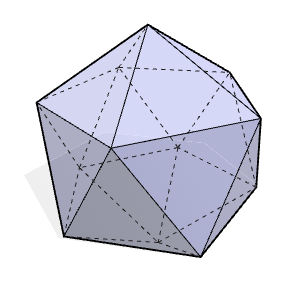
\includegraphics[width=0.3\textwidth]{figures/A0/icosahedron.png}
    \caption{Icosahedron. Figure from course note.}
    \label{fig:icosahedron}
\end{figure}
\begin{proof}
    Since we only care about the asymptotic behavior, we can ignore boundary vertices. Also, it's appropriate to approximately assume that the link $Lk(i)$ of every vertex $i$ is a icosahedron, as shown in \autoref{fig:icosahedron}:

    \begin{enumerate}
        \item Vertex $i$ has 12 valance, as well as all other vertices in the mesh. Since each valance (edge) is shared with 2 vertices, we have $E = \frac{12}{2} V \Rightarrow \frac{V}{E} = \frac{1}{6}$.
        \item Consider any edge that connects one vertex of the icosahedron and vertex $i$, it's shared with 5 triangle faces. Since each triangle face has 3 edges, we have $E = \frac{3}{5} F \Rightarrow \frac{F}{E} = \frac{5}{3}$.
    \end{enumerate}
    
    Divide $V - E + F - T = c$ with $E$ on both sides. As $E$ approaches infinity:

    \begin{equation}
        \lim_{E \rightarrow \infty} \frac{V - E + F - T}{E} = \lim_{E \rightarrow \infty} \frac{c}{E}
    \end{equation}
    \begin{equation}
        \Rightarrow \frac{V}{E} - 1 + \frac{F}{E} - \frac{T}{E} = 0
        \Rightarrow \frac{1}{6} - 1 + \frac{5}{3} - \frac{T}{E} = 0
        \Rightarrow \frac{T}{E} = \frac{5}{6}
    \end{equation}

    Therefore
    \begin{equation}
        \begin{cases}
            \frac{V}{E} = \frac{1}{6}\\
            \frac{F}{E} = \frac{5}{3}\\
            \frac{T}{E} = \frac{5}{6}
        \end{cases}
        \Rightarrow V:E:F:T = 1:6:10:5
    \end{equation}
\end{proof}

\emph{This ratio is roughly matched with the real examples in the course note.}

\section{Star, Closure, and Link}

$St(\mathcal S)$ is collection of all simplices $\sigma \in \mathcal K$ such that $\exists i \in \mathcal S, i \in \sigma$, as shown in \autoref{fig:ex8-st}:

\begin{figure}[h]
    \centering
    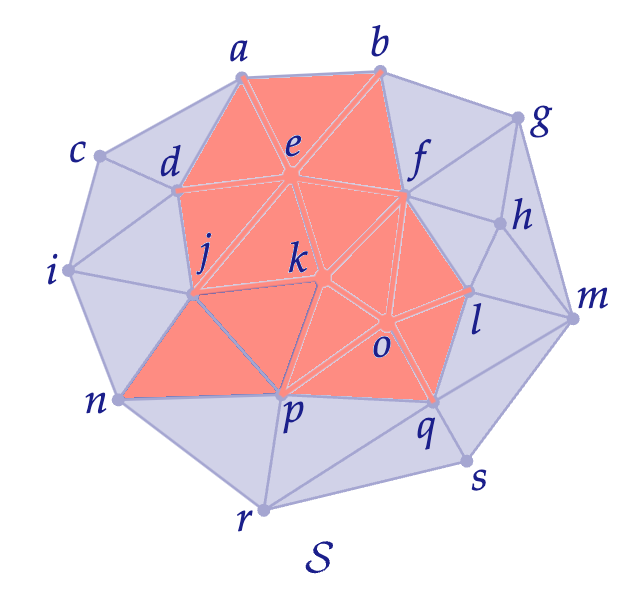
\includegraphics[width=0.3\textwidth]{figures/A0/ex8-st.png}
    \caption{$St(\mathcal S)$}
    \label{fig:ex8-st}
\end{figure}

$Cl(\mathcal S)$ is the smallest subcomplex of $\mathcal K$ containing $\mathcal S$, as shown in \autoref{fig:ex8-cl}:

\begin{figure}[h]
    \centering
    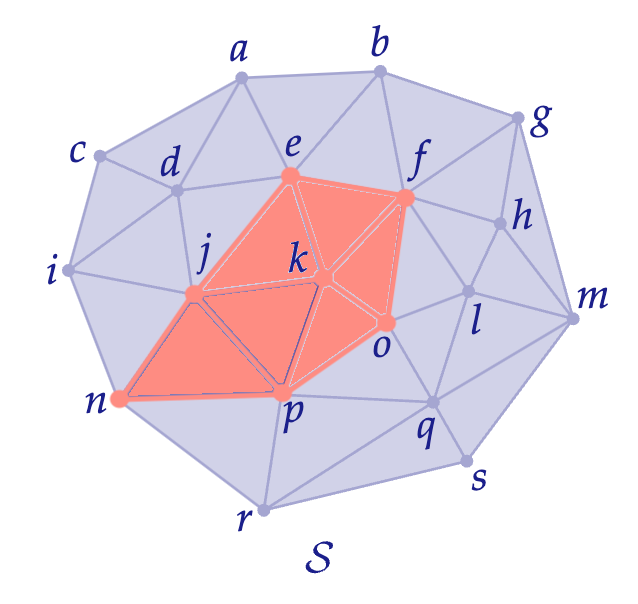
\includegraphics[width=0.3\textwidth]{figures/A0/ex8-cl.png}
    \caption{$Cl(\mathcal S)$}
    \label{fig:ex8-cl}
\end{figure}

To calculate $Lk(\mathcal S)$, $Cl(St(\mathcal S))$ and $St(Cl(\mathcal S))$ are needed, as shown in \autoref{fig:ex8-cl-st}. Then $Lk(\mathcal) = Cl(St(\mathcal S)) \ St(Cl(\mathcal S))$, as shown in \autoref{fig:ex8-lk}:

\begin{figure}[h]
    \centering
    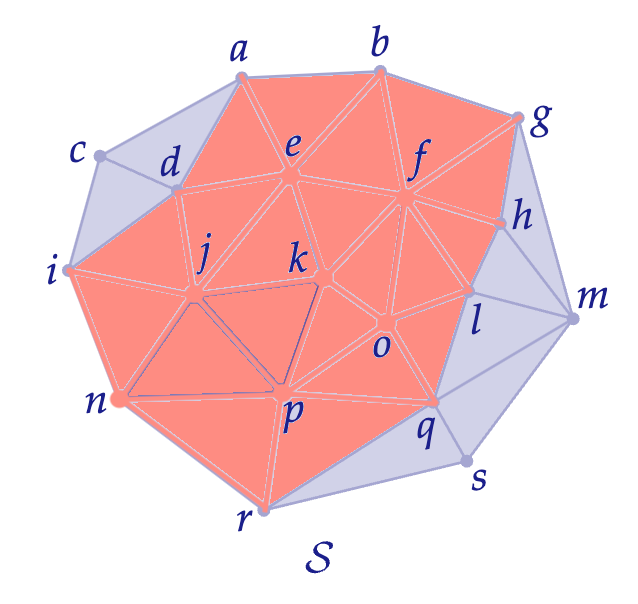
\includegraphics[width=0.3\textwidth]{figures/A0/ex8-cl-st.png}
    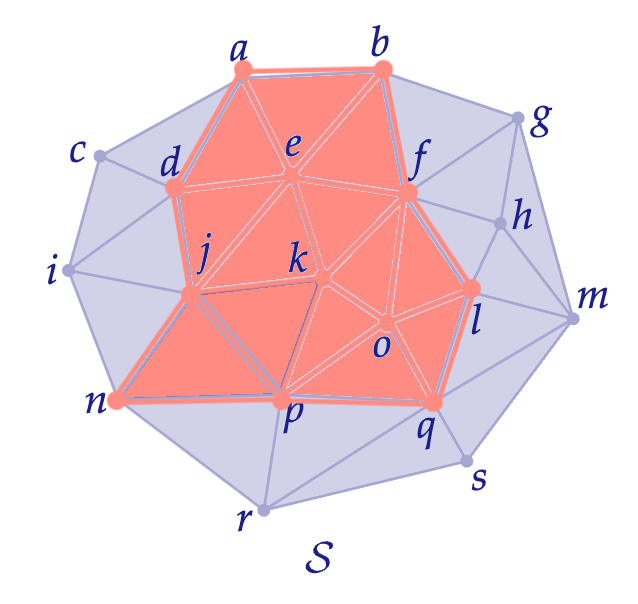
\includegraphics[width=0.3\textwidth]{figures/A0/ex8-st-cl.png}
    \caption{Left: $Cl(St(\mathcal S))$ Right: $St(Cl(\mathcal S))$}
    \label{fig:ex8-cl-st}
\end{figure}

\begin{figure}[h]
    \centering
    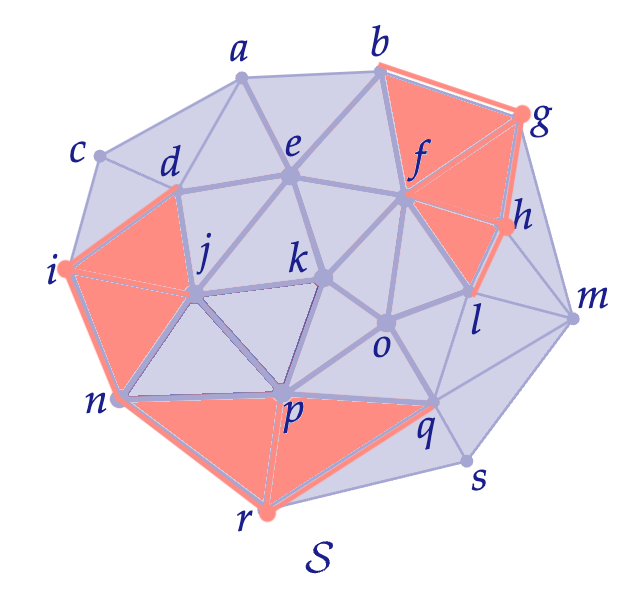
\includegraphics[width=0.3\textwidth]{figures/A0/ex8-lk.png}
    \caption{$Lk(\mathcal S)$}
    \label{fig:ex8-lk}
\end{figure}

\section{Boundary and Interior}

\section{Surface as Permutation}

\section{Permutation as Surface}

\section{Surface as Matrices}

\section{Classification of Simplicial 1-Manifolds}

\section{Boundary Loops}

\section{Boundary Has No Boundary}

